\input{preamble}

\begin{document}

\begin{titlepage}
  \begin{center}
    Министерство образования Республики Беларусь\\[1em]
    Учреждение образования\\
    БЕЛОРУССКИЙ ГОСУДАРСТВЕННЫЙ УНИВЕРСИТЕТ \\
    ИНФОРМАТИКИ И РАДИОЭЛЕКТРОНИКИ\\[1em]

    \begin{minipage}{\textwidth}
      \begin{flushleft}
        \begin{tabular}{ l l }
          Факультет & Информационных технологий и управления\\
          Кафедра   & Интеллектуальных информационных технологий
        \end{tabular}
      \end{flushleft}
    \end{minipage}\\[1em]

    \vspace{5em}


    \textbf{РАСЧЕТНАЯ РАБОТА}\\
    {по дисциплине <<Представление и обработка данных в интеллектуальных системах>>}\\
    на тему\\
    \textbf{\large Определить является ли граф кактусом}\\[1em]

    \vspace{10em}
    
    \begin{tabular}{ p{0.65\textwidth}p{0.25\textwidth} }
      Выполнил:& В.\,С.~Воинов \\[1em]
      Студент группы& \\
      421701 & \\
      Проверил: & Н.\,В.~Малиновская \\
     
    \end{tabular}
    
    \vfill
    {\normalsize Минск 2025}
  \end{center}
\end{titlepage} 

\pagenumbering{arabic}
\setcounter{page}{1}

\section{Введение}

\textbf{Цель: }Получить навыки формализации и обработки информации с
использованием семантических сетей

\textbf{Задача: }Определить является ли граф кактусом

\section{Список понятий}

\begin{enumerate}
\item
  \textbf{\textit{Граф}} - математическая абстракция реальной системы любой природы, объекты которой обладают парными связями. (совокупность точек, соединенных линиями. Точки называются вершинами, или узлами, а линии – ребрами, или дугами).

\begin{figure}[H]
  \centering
  
\includegraphics[scale=0.7]{img/graphs/graph.jpg}
  \caption{Граф}
\end{figure}


\item
  \textbf{\textit{Неориентированный граф }} — (абсолютное понятие) —  граф, в котором все ребра являются звеньями, то есть порядок двух концов ребра графа не существенен.
  \begin{enumerate}
  \item
    Вершина (относительное понятие, ролевое отношение);
  \item
    Связка (относительное понятие, ролевое отношение).
  \end{enumerate}

  \begin{figure}[H]
  \centering
  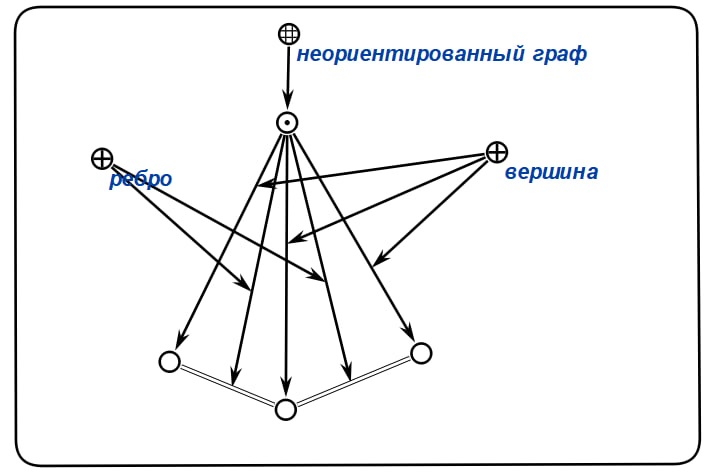
\includegraphics[scale=0.7]{img/graphs/neor.jpg}
  \caption{Неориентированный граф}
\end{figure}

  \item
  \textbf{\textit{Ребро неориентированного графа  }} —  это неупорядоченная пара вершин. В неориентированном графе рёбра не имеют направления. Это значит, что из любой вершины можно попасть в любую точку графа.

  \item
   \textbf{\textit{Граф-кактус }} — это связный неориентированный граф, в котором любой цикл (если есть) встречается не более одного раза, т.е. любое ребро принадлежит максимум одному циклу..

   \begin{figure}[H]
  \centering
  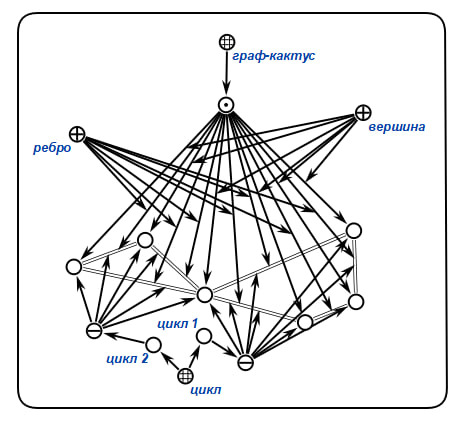
\includegraphics[scale=0.7]{img/graphs/cactus.jpg}
  \caption{Граф-кактус}
\end{figure}

\item 
\textbf{\textit{Цикл}} — это последовательность рёбер и вершин в графе, в которой, первая и последняя вершины совпадают, все рёбра и вершины (кроме начальной/конечной) различны, длина цикла больше или равна трём.
\end{enumerate}


\section{Тестовые примеры}

Во всех тестах графы будет приведены в сокращенной форме со скрытыми ролями элементов графа.

\subsection{Тест 1}

\textbf{Вход:}

Определить, является ли граф-кактусом.

\begin{figure}[H]
  \centering
  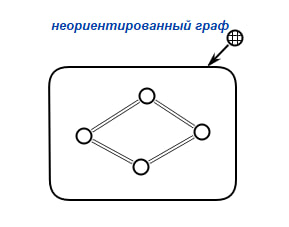
\includegraphics[scale=0.7]{img/test/test1.jpg}
  \caption{Вход теста 1}
\end{figure}

\textbf{Выход:}

Граф является графом-кактусом. 

\begin{figure}[H]
  \centering
  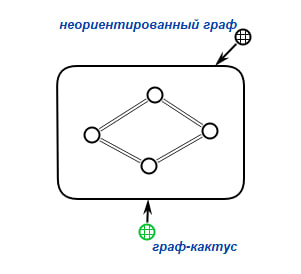
\includegraphics[scale=0.7]{img/vtest/vtest1.jpg}
  \caption{Выход теста 1}
\end{figure}

\subsection{Тест 2}

\textbf{Вход:}

Определить, является ли граф-кактусом.

\begin{figure}[H]
  \centering
  
\includegraphics[scale=0.7]{img/test/test2.jpg}
  \caption{Вход теста 2}
\end{figure}

\textbf{Выход:}

Граф не является графом-кактусом. 

\begin{figure}[H]
  \centering
  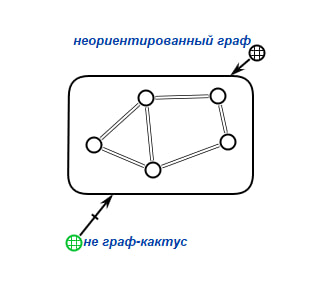
\includegraphics[scale=0.7]{img/vtest/vtest2.jpg}
  \caption{Выход теста 2}
\end{figure}

\subsection{Тест 3}

\textbf{Вход:}

Определить, является ли граф-кактусом.

\begin{figure}[H]
  \centering
  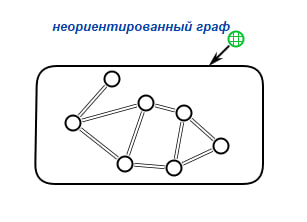
\includegraphics[scale=0.7]{img/test/test3.jpg}
  \caption{Вход теста 3}
\end{figure}

\textbf{Выход:}

Граф не является графом-кактусом. 

\begin{figure}[H]
  \centering
  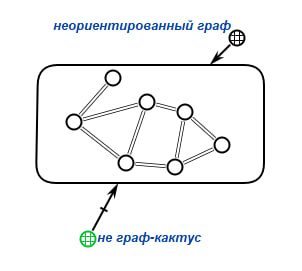
\includegraphics[scale=0.7]{img/vtest/vtest3.jpg}
  \caption{Выход теста 3}
\end{figure}

\subsection{Тест 4}

\textbf{Вход:}

Определить, является ли граф-кактусом.

\begin{figure}[H]
  \centering
  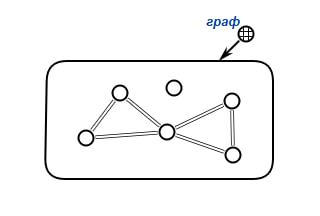
\includegraphics[scale=0.7]{img/test/test4.jpg}
  \caption{Вход теста 4}
\end{figure}

\textbf{Выход:}

Граф не является графом-кактусом. 

\begin{figure}[H]
  \centering
  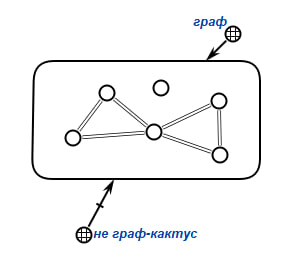
\includegraphics[scale=0.7]{img/vtest/vtest4.jpg}
  \caption{Выход теста 4}
\end{figure}

\subsection{Тест 5}

\textbf{Вход:}

Определить, является ли граф-кактусом. Рассмотрим граф из алгоритма.

\begin{figure}[H]
  \centering
  
\includegraphics[scale=0.7]{img/test/test5.jpg}
  \caption{Вход теста 5}
\end{figure}

\textbf{Выход:}

Граф является графом-кактусом. 

\begin{figure}[H]
  \centering
  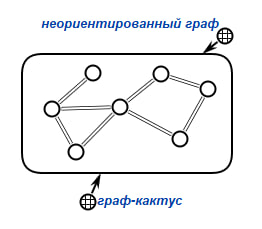
\includegraphics[scale=0.7]{img/vtest/vtest5.jpg}
  \caption{Выход теста 5}
\end{figure}



\section{Пример работы алгоритма в семантической памяти}

\begin{enumerate}
\item Шаг 1

\begin{figure}[H]
  \centering
  
\includegraphics[scale=1]{img/alg/alg1.png}
  \caption{Шаг 1}
\end{figure}

Задаем исходный неориентированный граф и начальную вершину. Создаем переменную visited, которая указывает на посещенную вершину графа.

\item Шаг 2

\begin{figure}[H]
  \centering
  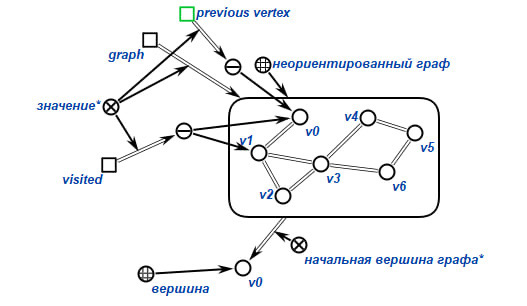
\includegraphics[scale=0.8]{img/alg/alg2.jpg}
  \caption{Шаг 2}
\end{figure}

Добавляем смежную вершину к текущей вершине в переменную visited. Запоминаем переход, создав переменную previous vertex, которой присваиваем только что посещённую вершину. 

\item Шаг 3 Повторяем процесс добавления ближайших смежных вершин до тех пор, пока все достижимые вершины не будут пройдены.

\begin{figure}[H]
  \centering
  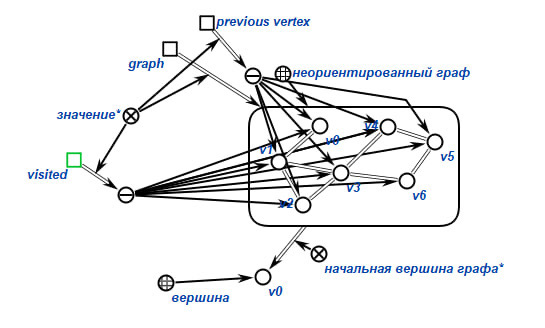
\includegraphics[scale=0.7]{img/alg/alg3.jpg}
  \caption{Шаг 3}
\end{figure}



\item  Шаг 4

\begin{figure}[H]
  \centering
  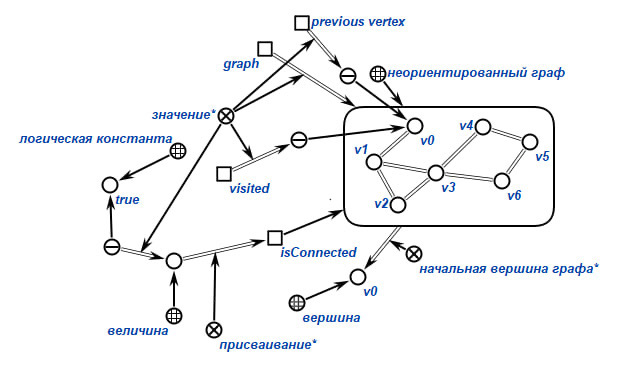
\includegraphics[scale=0.7]{img/alg/alg4.jpg}
  \caption{Шаг 4}
\end{figure}

Все вершины были посещены. Создаём переменную isConnected, которая хранит значение true. Это значит, что граф связный. Мы отбросили несвязные графы, которые точно не являются графами-кактусами. Обнуляем переменную previous vertex и visited, оставляем только начальную вершину.

\item Шаг 5

\begin{figure}[H]
  \centering
  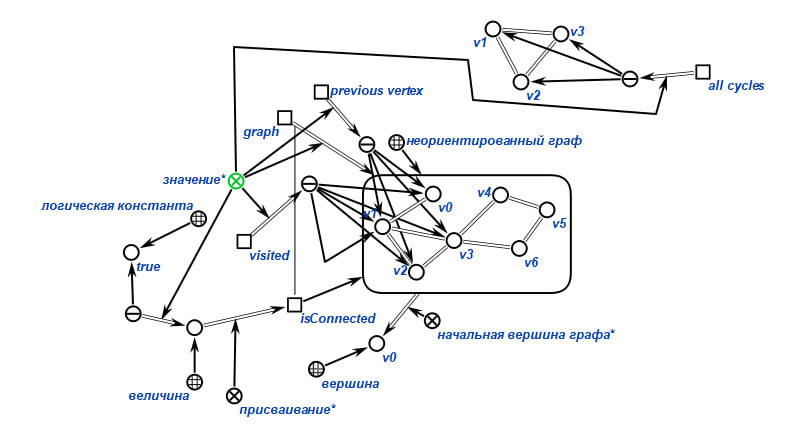
\includegraphics[scale=0.5]{img/alg/alg5.jpg}
  \caption{Шаг 5}
\end{figure}

Начинаем новый обход графа от начальной вершины. При каждом переходе сохраняем вершину в visited и обновляем previous vertex. Если в процессе обхода происходит возврат к вершине, которая уже присутствует в переменной visited, то это означает, что обнаружен цикл. Создаём переменную all cycles и добавляем туда найденный цикл в виде последовательности вершин, по которым был осуществлён возврат.

\item  Шаг 6 Повторяем процесс до тех пор, пока все достижимые вершины не будут пройдены.

\begin{figure}[H]
  \centering
  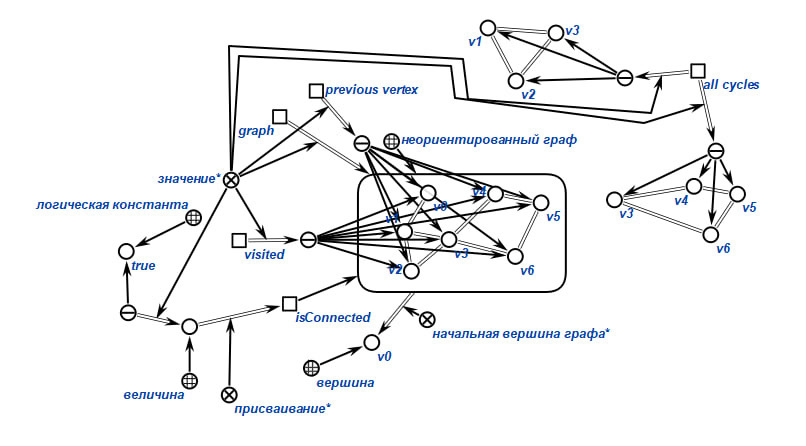
\includegraphics[scale=0.5]{img/alg/alg6.jpg}
  \caption{Шаг 6}
\end{figure}

\item Шаг 7

\begin{figure}[H]
  \centering
  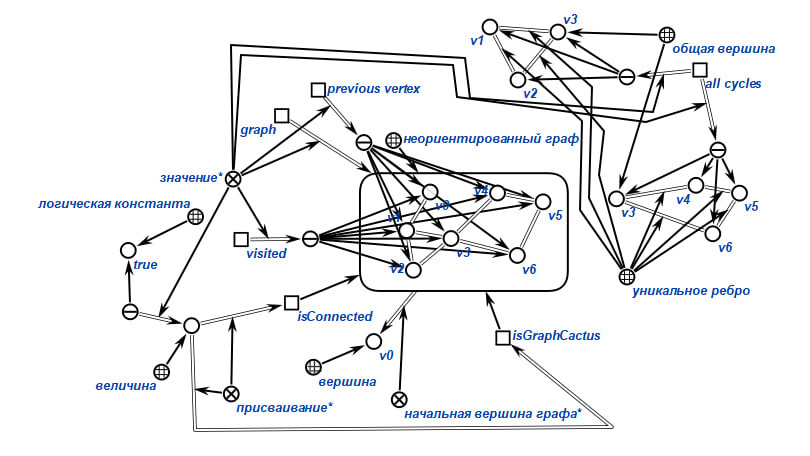
\includegraphics[scale=0.5]{img/alg/alg7.jpg}
  \caption{Шаг 5}
\end{figure}

Анализируем каждый цикл из переменной all cycles. Сравниваем циклы между собой и проверяем, не содержат ли они одно и то же ребро. Если находятся два цикла с общим ребром, делается вывод о том, что граф не является кактусом. В противном случае, если ни одно ребро не принадлежит двум и более циклам, а все вершины графа были посещены, делается вывод о том, что граф является кактусом.

\end{enumerate}

\newpage

\section{Заключение}
Был формализован алгоритм, построен фрагмент онтологии, продемонстрирована работа программы решения теоретико-графовой задачи по определению графов-кактусов в семантической памяти.
\newpage
\section{Литература}
\par [1] Емеличев В. А., Мельников О. И., Сарванов В. И., Тышкевич Р. И. Лекции по теории
графов. М.: Наука, 1990. 384с. (Изд.2, испр. М.: УРСС, 2009. 392 с.)
\vspace{1em}
\par [2] Оре О. Теория графов. – 2-е изд.. – М.: Наука, 1980. – С. 336.
\vspace{1em}
\par [3] https://youtu.be/vMFwwgtEZSI?si=7rIjlNZu8TH0lCU



% Если в тексте записки есть приложения, для добавления их в содержание, необходимо оставить слудеющую строку
% Если приложений нет - данную строку добавляем в комментарий
\addcontentsline{toc}{section}{Список использованных источников}

\nocite{*}
\selectlanguage{russian}
\bibliography{bibliography}


\end{document}